\section{Introduction}
The use of Optimal transport (OT) is now prevalent in many problem settings including information retrieval \citep{balikas2018cross,yurochkin2019hierarchical}, image processing \citep{otip}, statistical machine learning, as well as more recently, for ethics and fairness research \citep{kwegyiraggrey2021relative}. 
OT is well-suited for tasks where dissimilarity between two or more probability distributions must be quantified; 
its success was made possible through dramatic improvements in algorithms \citep{cuturi2013sinkhorn,solomon2015convolutional} that allow one to efficiently optimize commonly used functionals.
In practice, OT is often used to estimate and minimize the 
distance between certain (data-derived) distributions, 
using an appropriately defined loss functional. %Recent advances provide us the capability to drop-in and seamlessly integrate many types of losses into existing methods, for novel applications.
When one seeks to operate on more than two distributions, however, newer constructions are necessary to effectively estimate distances and transports.
To this end, a well studied idea in the literature is the ``barycenter,''
identified by minimizing the pairwise distance between itself and all other distributions given. 
The $d$-dimensional proxy distance is then defined as the sum of the distances to the barycenter.

%\begin{comment}
%\vikas{the following paragraph is low on content. Perhaps take 1-2 initial lines, compress and use it close off the previous paragraph?}
%The driving practical focus of optimal transport aims to estimate and minimize the distance between distributions of interest. Within machine learning, this takes the form of a loss; recent developments have enabled constructions of such a loss that allow almost seamless integration into existing methods. These incorporations have led to a number of benefits over traditional mean-squared error approaches, taking direct advantage of the statistical and distributional assumptions and requirements of the model fitter.
%\end{comment}

% {\bf Barycenters.} 
%While distances are defined between two points (or two probability distributions), barycenters extend the idea and enable analyzing many points (or probability 
% One way to quantify dissimilarity between many distributions is through distance to the mean. Here, for averaging,  
% we measure pairwise distances.
% Practically, this has led to models that can 
% concurrently enforce distributional similarity between a 
% set of distributions and has found use in 
% a spectrum of applications, which we will list shortly.

\textbf{Computing barycenters.}
Assuming that a suitably regularized form of the optimal transport loss is utilized, the pairwise distance 
calculation, by itself, can be efficient -- in fact, 
in some cases, Sinkhorn iterations can be used \citep{cuturi2013sinkhorn}. 
On the other hand, to minimize distances to the mean, 
most algorithms typically operate 
by repeatedly estimating the barycenter and those pairwise distances, and using a ``coupling'' strategy 
to push points toward the barycenter,
or in other cases, summing over all pairwise 
distances. 
% \glenn{I wonder if our method could be also more robust when the pairwise distances are very non-uniform, especially at early iterations...see  \href{https://www.stat.cmu.edu/~larry/=sml/Opt.pdf}  {https://www.stat.cmu.edu/~larry/=sml/Opt.pdf}at the end of page 10}\ronak{I like this idea, maybe we can allude to it briefly?}
%The idea is sensible but a
As the number of distributions 
grows, robustness issues can exacerbate \citep{alvarez2008trimmed} and the procedure is 
expensive (e.g., for 50 distributions, 50 bins).
%{\color{red}For example, even on a high end workstation, 
%simply computing the barycenter over
%50 distributions with 50 bins}
%does not converge within a reasonable number of iterations
%using newer packaged solvers. {\color{red} maybe instead of ``not...reasonable'', try ``not competitive"}
%is a time-intensive process.

% {\bf An efficient alternative.}
\textbf{A potential alternative.}
Multi-marginal optimal transport (MMOT) is a related problem to the aforementioned task but to some extent, the literature has developed in parallel.
In particular, MMOT focuses on identifying a joint distribution such that the marginals are defined by the input distributions over which we wish to measure the dissimilarity.
The definition naturally extends the two-dimensional formulation, and recent work has explored a number of applications \citep{pass2015multi}.
But the MMOT computation can be quite difficult,
and only very recently have practical algorithms been identified \citep{mmotcuturi}.
Additionally, even if a suitable method for computing an analogous measure of distance were available, 
\textit{minimizing} this distance to reduce 
dissimilarity (push distributions closer to each other) is practically hard if standard interior point solvers are needed just to compute the distance itself.
% however very recent research has shown that there exist polynomial time algorithms for this problem 
%have been shown to exist within the last year
% \cite{altschuler2021wasserstein}. Multimarginal versions of optimal transport have been studied but only few have led to practical algorithms \cite{mmotcuturi}.
% \vikas{can we concretize it 
% a little more? cite some numbers on a standard workstation? memory requirements? other resource needs?}
 %{\color{red} Glenn: fairness lead}

% {\color{red}this para does not add much}
% Importantly, we should also appreciate that the calculation of the barycenter is often a means to an end in most learning applications -- 
% the ultimate goal tends to be pushing these distributions to come closer. 
% A barycenter is a modeling choice, but other options may also be viable. 
% Indeed, if a different global measure of ``distributional disparity''
% were to be defined and minimized, the costs associated with pairwise comparisons and optimization
% may potentially be avoided. This hypothesis drives much of our development.

% \vikas{We need some work to justify the role/need of the following paragraph. What is the information is is designed to convey?} \glenn{I think we need to enforce this paragraph by contrasting it with our proposed approach, which I think its the intention of providing this information}
\noindent\textbf{Why and where is dissimilarity important?}
% {\color{red} START} Putting aside the cost to compute the barycenter for the moment, 
% instantiations of such applications often desire to enforce distribution similarity
% only on model outputs.
% For example, in \cite{jiang2020wasserstein}, the authors define fairness measures over the probability of the prediction given ground truth labels.  
% This choice is not without good reasons: discrete outputs lead to extremely nice distributions over the probability simplex, where optimization is easy and assumptions need not be strong.{\color{red} END; could START--END be replaced with the gray text?}
Enforcing distributions to be similar is a generic goal whenever one wishes some outcome of interest to be agnostic about particular groups within the input data.
In applications where training deep neural network models is needed,
% In applications,
it is often a goal to enforce distribution similarity on model outputs. 
For example, in \cite{jiang2020wasserstein}, the authors define fairness measures over the probability of the prediction, given ground truth labels.   
%FIXME: if you read this and know what X Y and Z are, then fill in and uncomment. This leads to distributions over the probability simplex with the desirable qualities X, Y and Z.
% 
However, these methods are rarely extended to continuous measures 
among internal neural network activations,
%(e.g., Bayesian networks), 
mainly due to the strong distributional assumptions needed (product of Gaussians) and the added algorithmic complexity of estimating the barycenter.
These issues limit application of these ideas 
%assumption-free distribution enforcement 
to only the final outputs of neural network models, where the distribution is typically binomial or multinomial.
% One drawback of this choice means that the distributional closeness is only guaranteed over the global model output {\vikas: this is unclear}, and little can be said about layer outputs prior to the thresholding for prediction.
MMOT solutions might be employed here, but suffer similar computational limitations.
% Additionally, full retraining would be necessary if thresholds must be adjusted due to changing business or regulatory requirements.

\noindent\textbf{Contributions.}  \textbf{(1)} We identify a particular form of the discrete multi-marginal optimal transport problem
which admits an extremely fast and numerically robust solution.
Exploiting a recent extension of 
the classical Earth Movers Distance (EMD) to a higher-dimensional Earth Mover's objective,
we show that such a construction is equivalent
to the discrete MMOT problem with Monge costs.
\textbf{(2)} We show that minimization of this \textit{global} distributional measure
leads to the 
harmonization of input distributions very similar in spirit to the minimization of distributions to barycenters (see Figure~\ref{fig:hists}).
\textbf{(3)} We prove theoretical properties of our scheme, and show that 
the gradient can be read directly off from a primal/dual algorithm,
alleviating the need for 
computationally intense 
pairwise couplings needed for barycenter approaches.
\textbf{(4)} The direct availability of the gradient
enables a specific neural network instantiation,
and
with a particular scaffolding provided by differentiable histograms, 
we can operate directly on network activations (anywhere in the network) to compute/minimize the d-MMOT. 
%The proposal integrates nicely with 
%existing pipelines. 
We establish via experiments that computing gradients used in backpropagation is fast, due to rapid access to solutions of the dual linear program.
We compare with barycenter-like approaches in several settings, including common fairness applications.
%, and show that our proposal 
%Our final construction,
%the $d$-dimensional Earth Mover's Distance (DEMD),
%integrates nicely with existing neural network pipelines. 

\begin{figure}[t]
    \centering
    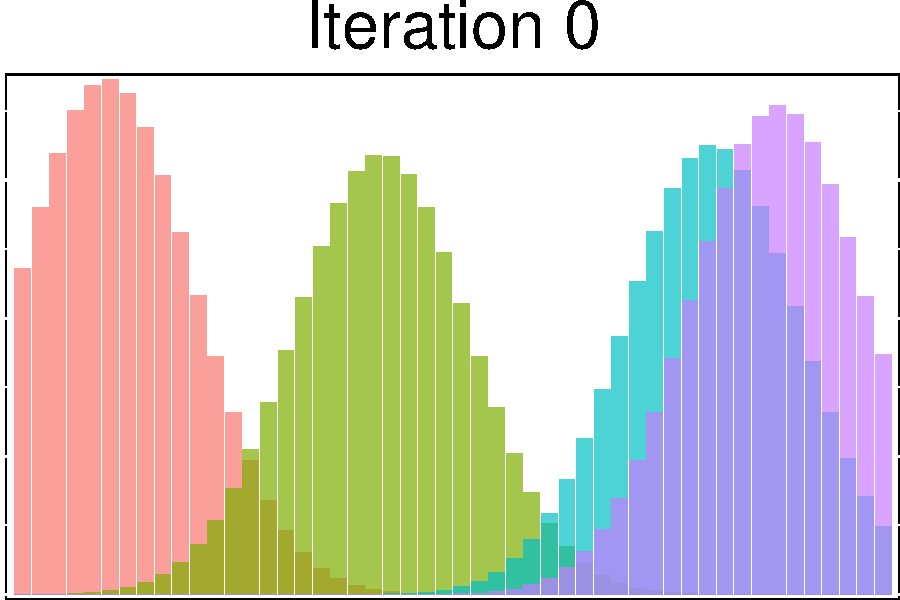
\includegraphics[width=0.19\textwidth]{6_demd/figs/hists/hists_iter_0.pdf}
    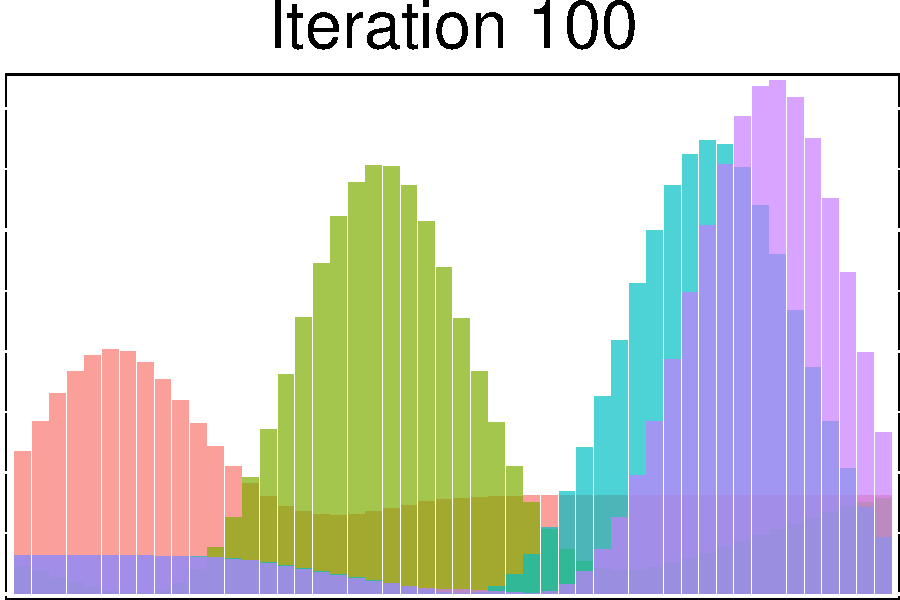
\includegraphics[width=0.19\textwidth]{6_demd/figs/hists/hists_iter_100.pdf}
    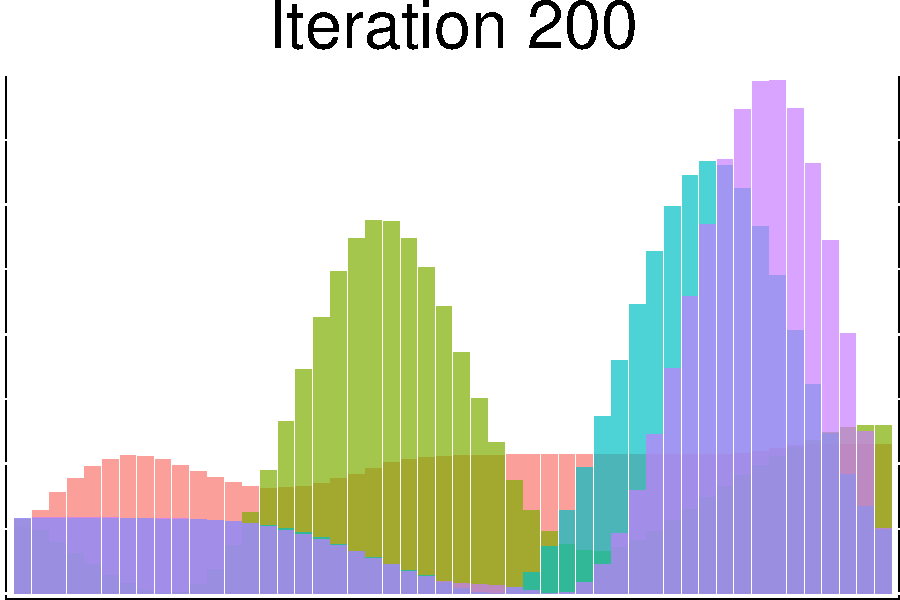
\includegraphics[width=0.19\textwidth]{6_demd/figs/hists/hists_iter_200.pdf}
    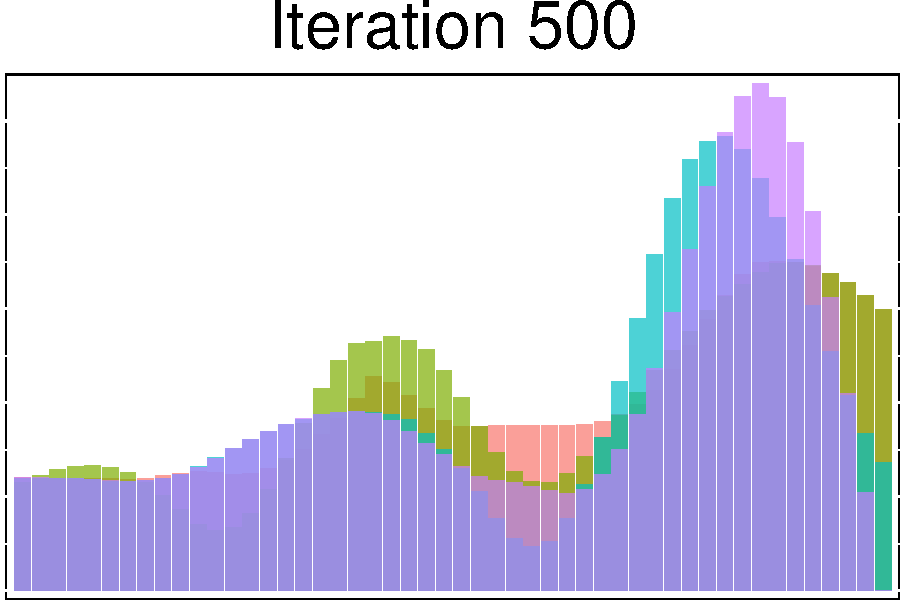
\includegraphics[width=0.19\textwidth]{6_demd/figs/hists/hists_iter_500.pdf}
    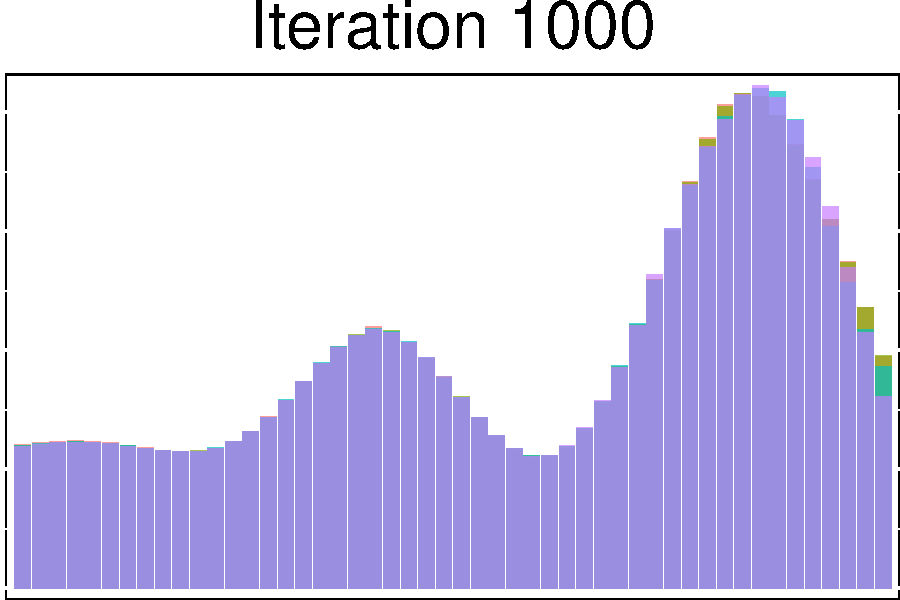
\includegraphics[width=0.19\textwidth]{6_demd/figs/hists/hists_iter_1000.pdf}
    \caption{\footnotesize Starting and ending state of minimizing a multi-marginal OT distance. Each iteration minimizes the generalized Earth Mover's objective, and then updates each histogram in the direction provided by the gradient.}
    \label{fig:hists}
    \vspace{-10pt}
\end{figure}

%%%% OLD
% In this work, we identify a simple {\em global} distributional measure with scaffolding that allows for fast computation over any continuous model output. A new multi-dimensional generalization of the classical Earth Mover's distance has recently been shown to be efficiently computable, and further developments show  that its minimization is extremely fast compared to existing barycenter-style methods.
% Functionally, it
% possesses several useful ingredients: (a) it requires no distributional assumptions, (b) it is efficient to compute, (c) its gradient is also efficiently computable. As a result, the functional can be 
% directly used in regimes where gradients are required for optimization (e.g., backpropogation and other gradient descent methods). 
% Finally, the functional is  numerically stable, and has an intuitive interpretation which facilitates interpretative reasoning.  
% In this work, we identify a simple {\em global} distributional measure with scaffolding that allows for fast computation over any continuous model output. A new multi-dimensional generalization of the classical Earth Mover's distance has recently been shown to be efficiently computable, and further developments show  that its minimization is extremely fast compared to existing barycenter-style methods. Functionally, it
% %distributions are computed over the invariant sets, a barycenter is computed as for the measure of invariance, and heuristic methods are employed to reducing the measured invariance in the loop. 
% Although these approaches aim to directly address the heterogeneity in the model output, they require (1) particular algorithms and solvers for relaxing discrete outputs to enable backpropogation and (2) that operating points and thresholds determining the final prediction are fixed. 
% If a method to operate directly on the activations prior to thresholding was feasible...
% Operating directly on the activations has its own hurdles.
% The activations are continuous, and so distributional assumptions must be made if any computation in the learning pipeline is to remain tractable. However a priori these assumptions are explicitly unknown. 
% \vikas{this appears to be tailored to the above paragraph. Ideally, we should start by highlighting a feature that allows moving away from the pairwise iterative scheme of barycenters.}
% In this work, we observe that a \textit{discretization} of continuous layer outputs allows for the computation of a new multi-distributional generalization of the classical Earth Mover's Distance (EMD) that allows for drop-in computation of disparity at the activation-level. 
% A common application of optimal transport incorporates the concept into a machine learning model by appending a suitable regularization term to the model's objective function.  Typically, this regularization term has the effect of making the statistical distribution of subsets of solutions either more uniform or else invariant in some prescribed way.  An illustration of a prototypical process appears in Figure~\ref{fig:hists}.
% In this paper, we apply a multi-distributional generalization of the classical Earth Mover's distance to the task of regularizing network models.
% The generalization that we employ is based on the classical Earth Mover's Distance (EMD), and
% We demonstrate that this functionally 
% possesses several useful ingredients: (a) it requires no distributional assumptions, (b) it is efficient to compute, (c) its gradient is also efficiently computable. As a result, the functional can be 
% directly used in regimes where gradients are required for optimization (e.g., backpropogation and other gradient descent methods). 
% Finally, the functional is  numerically stable, 
% and has an intuitive interpretation which facilitates interpretative reasoning.  
% Empirical demonstrations of the speed and viability of our approach are presented in Section~\ref{sec:results}.
% We take direct advantage of linear programming formulations of the EMD in its generalized form, and show that in fact the gradient can be directly identified as the solution to the dual program. Recent algorithmic developments allow for the primal and dual to be solved concurrently, allowing for a no-cost gradient computation if the forward computation is chosen accordingly.
% Whereas the classical Earth Mover's distance defines a distance metric between pairs of distributions, the generalized Earth Mover's objective defines a natural way to  measure  dissimilarity amongst $d\geq 2$ distributions. 
% Both the classical distance and the generalized objective can be expressed as linear programs.
% One advantage of the linear program formulation is the fact that every linear program has an equivalent {dual} linear program.
% We demonstrate, using standard sensitivity analysis, that solutions to the dual linear program equal the primal objective functional's gradient. If the functional is regularizing a neural network model, this gradient can be used for backpropagation of derivatives during model training.
% Additionally, it was recently shown that solving both the primal and dual linear programs of the generalized Earth Mover's objective can be accomplished in linear time and constant space by applying a straightforward  greedy algorithm. In experiments, we compare the speed to compute the gradients of the generalized Earth Mover's objective of the greedy algorithm against native auto-gradient procedures, and we demonstrate over $1000$-fold speed improvement. The method we describe is numerically stable, as no division operations or unusually large quantities are invoked in the process of solving the linear programs.  
% In many settings, however, a strict set of assumptions is required to apply and compute these existing methods. Particularly, optimal transport measures over continuous spaces are only practical when strong distributional assumptions can be made, and while discrete assumptions allow for more broad computation, they tend to poorly capture and generalize the actual measures of interest.
% An important feature of our approach is that it acts on model outputs prior to thresholding, so invariances to be maintained across varying thresholds.
% Our procedure addresses both of these limitations directly, by first promoting invariance at all discretizations of model outputs \textit{prior to thresholding}, and by making use of a differentiable histogramming procedure to directly apply precomputed gradients through backpropagation.
% A challenge in practical implementations that use this architecture  define invariance can be based on business or regulatory constraints, but these constraints can change over time.  Industry deployments of ML pipelines are not compatible with such a setting is an important way: thresholds considered for discretization or classification are often adjusted or changed due to changing business or regulatory directives.   After training with procedures similar to the above, no guarantee regarding invariance can be made if the threshold is changed. It is often not sufficient or even feasible to retrain when operating points may or must change.
% {\color{red} redundant, merge with above para}
% \noindent\textbf{Contributions.} In this work, we present an application of a recent extension of the classical Earth Movers distance to a higher-dimensional Earth Mover's objective.
% We show that minimization of the objective leads to the harmonizing (lang) of input distributions similar to the minimization of distributions to barycenters.
% We prove theoretical properties of the objective and the procedure that
% reveals the gradient can be read directly off from a primal/dual algorithm,
% alleviating the need for computing intensive pairwise couplings.
% % This objective provides an alternative to barycenter approaches as a way to regularize network models in a way that reduces statistical dissimilarity of the optimal solutions. % The functional we use acts on a \textit{discretized version} of model outputs prior to thresholding, and allows for invariances to be maintained across varying thresholds. 
% With a particular instantiation of differentiable histograms, we can apply and smoothly operate directly on network activations to compute the EMD measure. 
% We establish through experiment that the speed of computing gradients used in backpropogation can be computed in substantially shorter times than one can achieve using standard tools, due to rapid access to solutions of the the dual linear program formulation.
% We compare and contrast the performance and speed of our construction against Barycenter-like measures in a number of settings and demonstrate applications in a common fairness setting.
% Our final construction integrates seamlessly with existing neural network pipelines.
% Machine learning has become ubiquitous, but has suffered some setbacks in public and regulatory visions due to issues typically considered orthogonal to traditional measures of success within the literature.
% Most modern advancements in machine learning follow from learning a model that optimizes for some measure of \textit{accuracy}, measured by misclassification errors over all samples or global measures of true and false positive and negative rates.
% Unfortunately, when statistical assumptions of homogeneous data fail, these measures can be skewed heavily towards subsets of the data that follow a majority or the primary mode of the underlying distribution. These biases can take many forms, and in applications in which data and outcomes may be represent people and decisions for those people, can lead directly towards unfairness and disparity among groups.
% The last few years of machine learning deployment has revealed a myriad of situations in which strong bias and fairness concerns have led to strong social backlash. Examples: COMPAS, twitter, etc. \cite{?}
% With these concerns has also come interest in technical solutions to fairness and bias. Several conferences and workshops have been created \cite{fat, facct, etc}, devoted to grounding and understanding these ideas within a mathematical and statistical context. From these communities concrete definitions have been formed, along with a number of algorithmic solutions to both avoid and account for bias and unfairness within both data and models.
% Existing methods for accounting for fairness typically define measures over discrete output spaces, and attempt to minimize some measure of disparity between these discrete probabilities. Varying definitions of fairness have been constructed under this umbrella, and a number of nice solutions have been proposed that allow for fair regularization in traditional machine learning training pipelines.
% A drawback to these approaches is that they rely on the discrete/binary outputs of models to be fixed: once a model is trained, the threshold used for those outputs cannot be changed else all fairness guarantees provided by the regularization fail, because the output distributions have all been constructed with that specific threshold. Practical deployments of machine learning models in industry rely on being able to select different points of operation, to match secondary requirements or measures provided by business or regulatory requirements. In these cases it is not sufficient or feasible, especially for large models, to create and retrain methods when these operating points must change. Their is a clear need for methods which are fair across potentially many points of operation.
% While moving to fairness over the continuous measure prior to thresholding may be infeasible, new results suggest that discretization at points of operation can lead to practical solutions for constructing models fair over many thresholds.
% \noindent\textbf{Contributions.} In this work, we analyze fairness from a new perspective. By looking at the distances between distributions over discretized spaces prior to thresholding for downstream discrete tasks, we apply a recently developed tool for computing EMD distance to quickly measure the disparity between groups over discretized continuous measures. Using a key observation that the gradients are readily available, we directly incorporate this EMD distance into standard machine learning pipelines. 